\label {fs-acker-experiments}

We have tested the \tracker\ performance on a simple directed path graph of various length, which was shuffling processed elements between machines in each vertex. The \tracker\ of various configurations was compared with tracking using markers and no tracking at all. Elements were tracked in windows of 1, 10 and 100.
Virtual machines used in experiments had single CPUs and 4 GB of RAM per machine. One machine called a Bench Stand was used to input data into the dataflow at a fixed rate while measuring the speed of it being processed via receiving output and notifications for data being processed. \tracker\ was running on machines excluded from the dataflow: a single one for centralized configuration and two for distributed configuration.

\subsection{Network traffic}

Network traffic was measured in number of separate service messages sent over the network. Local \tracker\ was sending messages in batches.

% https://gist.github.com/faucct/032aaf6240db361d30a184b1d7bf3c8e
\begin{figure*}[t!]
    \begin{subfigure}[b]{0.32\textwidth}
            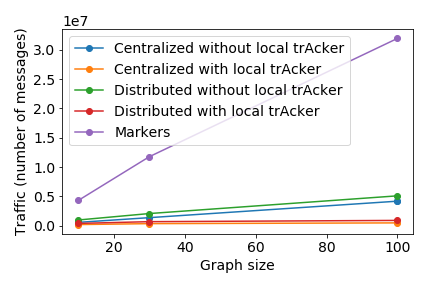
\includegraphics[width=0.99\textwidth]{pics/traffic_by_graph_size.png}
            \caption{Traffic by graph size}
    \end{subfigure}
    \hspace{5mm}
    \begin{subfigure}[b]{0.32\textwidth}
            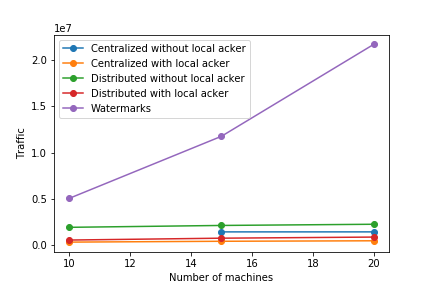
\includegraphics[width=0.99\textwidth]{pics/traffic_by_number_of_machines.png}
            \caption{Traffic by number of virtual machines}
    \end{subfigure}
    \hspace{5mm}
    \begin{subfigure}[b]{0.32\textwidth}
            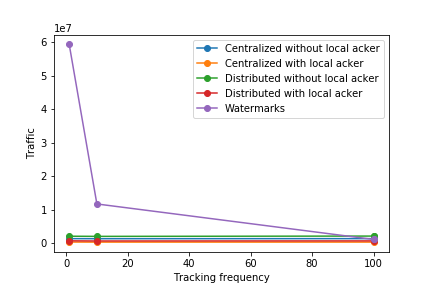
\includegraphics[width=0.99\textwidth]{pics/traffic_by_tracking_frequency.png}
            \caption{Traffic by tracking frequency}
	\end{subfigure}
    \caption{Service traffic of various trackings}
\end{figure*}

\subsection{Notification latency}

Notification latency was measured as a time between moments of Bench Stand receiving last elements in tracking windows and notifications for that window.

% https://gist.github.com/faucct/032aaf6240db361d30a184b1d7bf3c8e
\begin{figure*}[t!]
    \begin{subfigure}[b]{0.32\textwidth}
            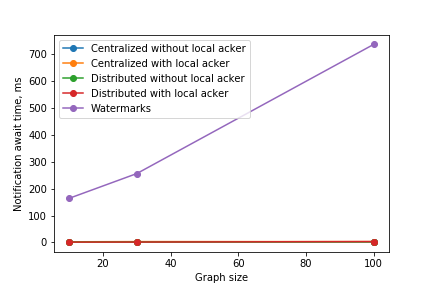
\includegraphics[width=0.99\textwidth]{pics/notification_await_time_by_graph_size.png}
            \caption{Notification latency by graph size}
    \end{subfigure}
    \hspace{5mm}
    \begin{subfigure}[b]{0.32\textwidth}
            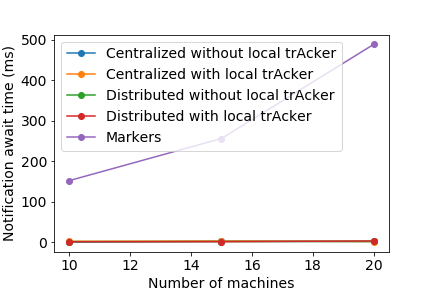
\includegraphics[width=0.99\textwidth]{pics/notification_await_time_by_number_of_machines.png}
            \caption{Notification latency by number of virtual machines}
    \end{subfigure}
    \hspace{5mm}
    \begin{subfigure}[b]{0.32\textwidth}
            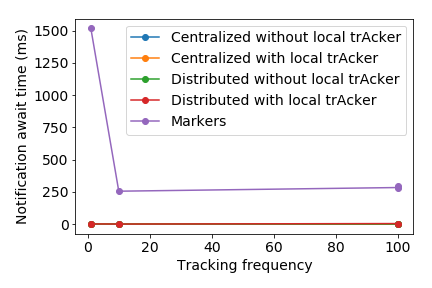
\includegraphics[width=0.99\textwidth]{pics/notification_await_time_by_tracking_frequency.png}
            \caption{Notification latency by tracking frequency}
	\end{subfigure}
    \caption{Notification latency of various trackings}
\end{figure*}

\subsection{Scalability}

In those experiments we are reproducing a case in which the centralized \tracker\ was not holding the load, while the distributed \tracker\ was working. We have failed to reproduce it while using 100 machines running our dataflow. Still, we have been able to simulate it by increasing the total number of Ack messages.

% https://gist.github.com/faucct/546f5617b958349a125449926373b780
\begin{figure}[htbp]
  \centering
  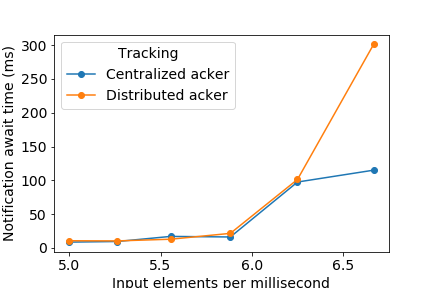
\includegraphics[width=0.50\textwidth]{pics/scalability_01x.png}
  \caption{1x acks}
\end{figure}
\begin{figure}[htbp]
  \centering
  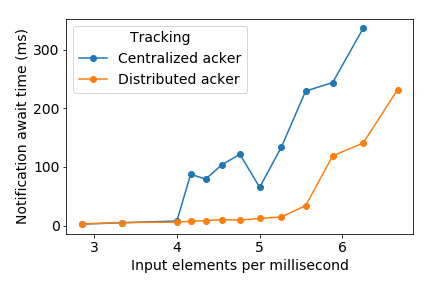
\includegraphics[width=0.50\textwidth]{pics/scalability_05x.png}
  \caption{5x acks}
\end{figure}
\begin{figure}[htbp]
  \centering
  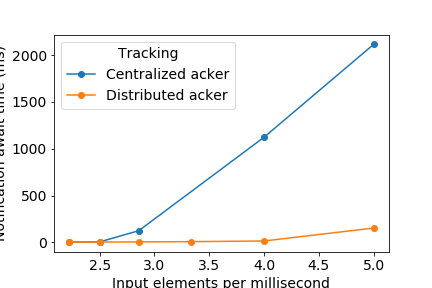
\includegraphics[width=0.50\textwidth]{pics/scalability_09x.png}
  \caption{9x acks}
\end{figure}
\begin{figure}[htbp]
  \centering
  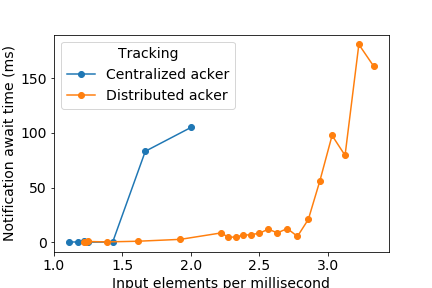
\includegraphics[width=0.50\textwidth]{pics/scalability_17x.png}
  \caption{17x acks}
\end{figure}

\subsection{Overhead on throughput}

In those experiments we compare maximum throughput of system without tracking to systems with various trackings. \tracker's overhead on maximum throughput is not substantial and does not depend on tracking window frequency. Overhead of tracking with markers is huge when tracking every element.

\begin{figure}[htbp]
  \centering
  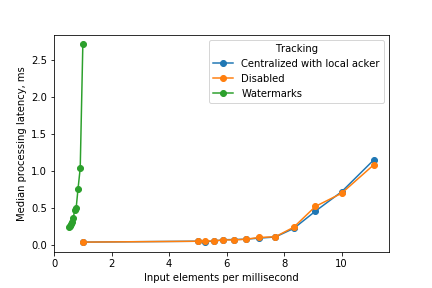
\includegraphics[width=0.50\textwidth]{pics/throughput_overhead.png}
  \caption{Throughput overhead}
\end{figure}

\subsection{State snapshotting}

In those experiments we are comparing granular tracking using \tracker\ and markers. Processed elements are divided into snapshot windows. Pipeline vertices only process elements from a current snapshot window and buffer ones from a next snapshot window until they receive a notification that all elements from a current snapshot have been processed. When this happens vertices imitate snapshotting with a fixed duration sleep and continue to process elements from next snapshot window. We have measured a number of buffered elements and total time they have spent in buffer varying the snapshot duration.

% https://gist.github.com/faucct/6097d9d08197cb979b71721b16f8b6a3/
\begin{figure}[htbp]
  \centering
  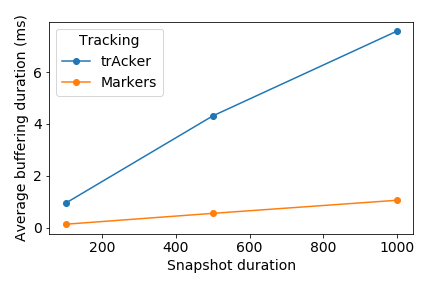
\includegraphics[width=0.50\textwidth]{pics/buffering_average_duration.png}
  \caption{Average buffering duration}
\end{figure}
\begin{figure}[htbp]
  \centering
  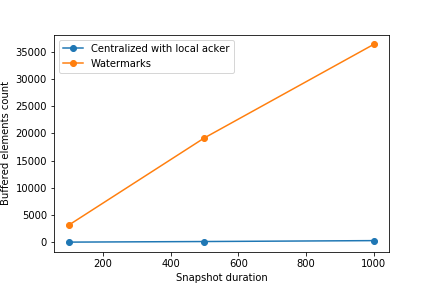
\includegraphics[width=0.50\textwidth]{pics/buffering_count.png}
  \caption{Buffered elements count}
\end{figure}
\begin{figure}[htbp]
  \centering
  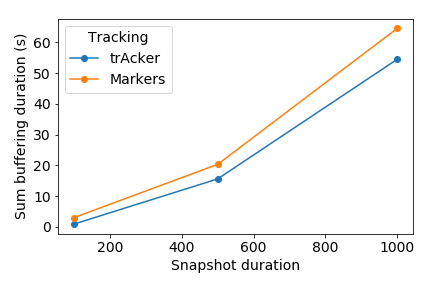
\includegraphics[width=0.50\textwidth]{pics/buffering_sum_duration.png}
  \caption{Total buffering duration}
\end{figure}
\begin{figure}[htbp]
  \centering
  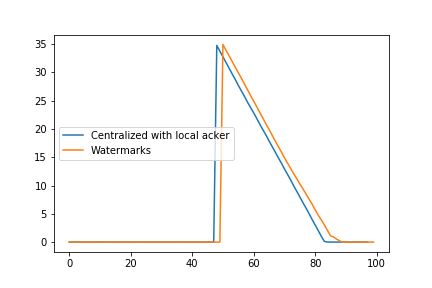
\includegraphics[width=0.50\textwidth]{pics/buffering_latencies_evolution_acker.png}
  \caption{Latencies with \tracker}
\end{figure}
\begin{figure}[htbp]
  \centering
  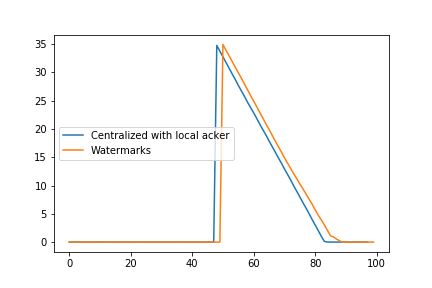
\includegraphics[width=0.50\textwidth]{pics/buffering_latencies_evolution_watermarks.png}
  \caption{Latencies with markers}
\end{figure}

\subsection{Count iterations?}

